\documentclass[12pt]{article}

% Specify how big is going to be the paper margins.
\usepackage[a4paper, margin=1in]{geometry}

% amsmath: Add useful commans like aligh and gather.
% amsfonts: Add useful fonts like \mathbb{R}.
% amssymb: Add useful symbles like \therefore (needs amsfonts to work).
\usepackage{amsmath, amsfonts, amssymb}

% Makes the use of colors possible.
\usepackage{xcolor}

\definecolor{color1}{HTML}{0e4a7a}
\definecolor{color2}{HTML}{1282d6}
\definecolor{color3}{HTML}{7ac1ff}

% Add Latin Modern Fonts like Sans-serif and Roman.
\usepackage{lmodern}

% Makes header and footer configurable.
\usepackage{fancyhdr}

% Makes the use of colored and configured tables possible
\usepackage[most]{tcolorbox}

% Add commands to specify theorems like \newtheorem{x}{y}.
\usepackage{amsthm}

% Enables enumeration of items.
\usepackage{enumitem}

% Enables adding images.
\usepackage{graphicx}

% Enables cool hyper references.
\usepackage[colorlinks=true, linkcolor=color2, urlcolor=color2, citecolor=color2]{hyperref}

\title{\sffamily\bfseries{Soluções Jacob Palis 2022 N2}}
\author{Samuel de Araújo Brandão}
\date{4 de Setembro de 2025}

\pagestyle{fancy}
\fancyhf{}

\fancyhead[L]{\sffamily\bfseries{Soluções Jacob Palis 2022 N2}}
\fancyhead[R]{\textcolor{color2}{Samuel Brandão}, 4 de Setembro de 2025}
\fancyfoot[C]{\thepage}
\setlength{\headheight}{14.5pt}

\tcbset{
  statementbox/.style = {
    enhanced,
    width=\textwidth,
    title={Enunciado},
    title filled,
    fonttitle=\sffamily\bfseries,
    coltitle=white,
    colbacktitle=color1,
    colback=white,
    colframe=color1,
    boxrule=1pt,
    arc=2mm,
    boxsep=2pt,
  }
}

\tcbset{
  theorembox/.style = {
    enhanced,
    width=\textwidth,
    colback=white,
    colframe=color1,
    boxrule=1pt,
    arc=2mm,
    boxsep=2pt
  }
}

\tcbset{
  lemmabox/.style = {
    enhanced,
    width=\textwidth,
    colback=white,
    colframe=color2,
    boxrule=1pt,
    arc=2mm,
    boxsep=2pt
  }
}

\renewcommand*\contentsname{\textsf{Conteúdos}}
\newcommand{\kb}[1]{\left\lfloor #1 \right\rfloor}

\begin{document}
  \maketitle
  Uma coleção de soluções para a \textbf{Jacob Palis 2024 Nível 2}, inspirada no estilo de Evan Chen.
  Pode-se encontrar todos os problemas e respostas oficiais 
  \textbf{\href{https://www.obm.org.br/content/uploads/2024/06/jacob_palis_2024_provas_e_solucoes.pdf}{aqui}}.

  Todas as soluções foram inteiramente escritas por mim, enquanto me preparava para a
  International Mathematical Olympiad (IMO).

  Caso encontre algum erro ou tiver sugestões ou comentários, sinta-se a vontade 
  para entrar em contato!

  \tableofcontents

  \clearpage

  \section{\textsf{Problemas}}
    \subsection{Testes}
      \begin{enumerate}[label=\textbf{\arabic*.}]
        \item Sejam \(x, y, z, w\) inteiros positivos tais que \(20^{24} = 2^x \cdot 5^y = 8^z \cdot 25^w\). Qual é o valor de \(x + y + z + w\)?
        \item Lucas estava participando de uma corrida de rua de 21 quilômetros e olhando sempre o tempo médio por quilômetro. Ao final do
          quilômetro 14 o seu tempo médio era de 6 minutos e 42 segundos por quilômetro. Nos últimos 7 quilômetros o ritmo dele baixou e ele
          concluiu o quilômetro 21 com tempo médio de 6 minutos e 50 segundos por quilômetro no percurso completo. Qual foi o tempo médio de
          Lucas nos últimos 7 quilômetros?
        \item Qual o número máximo de meses com 5 quintas-feiras que um ano pode ter?
        \item Quantos triângulos na figura abaixo têm soma de seus números par?
          \begin{figure}[h]
            \centering
            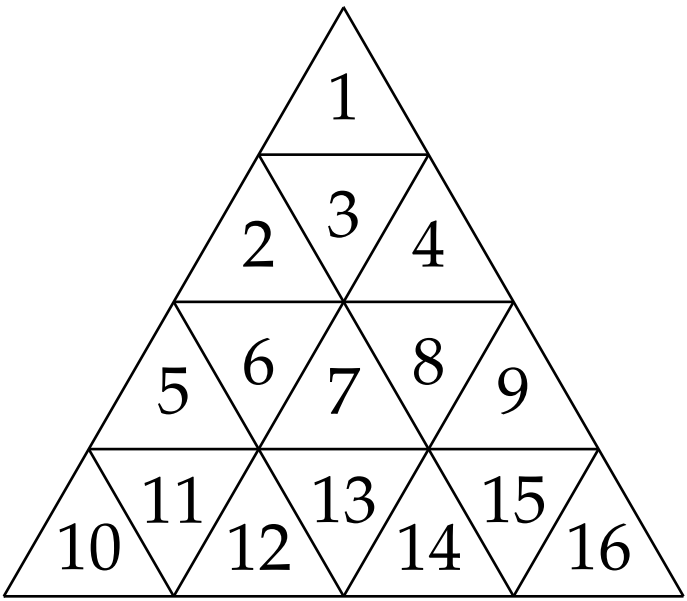
\includegraphics[width=0.3\textwidth]{first.png}
          \end{figure}
        \item Na figura a seguir no interior de um retângulo há um pentágono regular, um triângulo equilátero e um
quadrado. Os três polígonos regulares possuem um vértice em comum, os outros dois vértices do triângulo
equilátero estão sobre os lados do pentágono e do quadrado e o pentágono e o quadrado possuem um vértice
sobre os lados do retângulo. Sabe-se que lados do pentágono e do quadrado formam ângulos com medida x
com lados opostos do retângulo (como na figura). Quanto vale x em graus? 
          \begin{figure}[h]
            \centering
            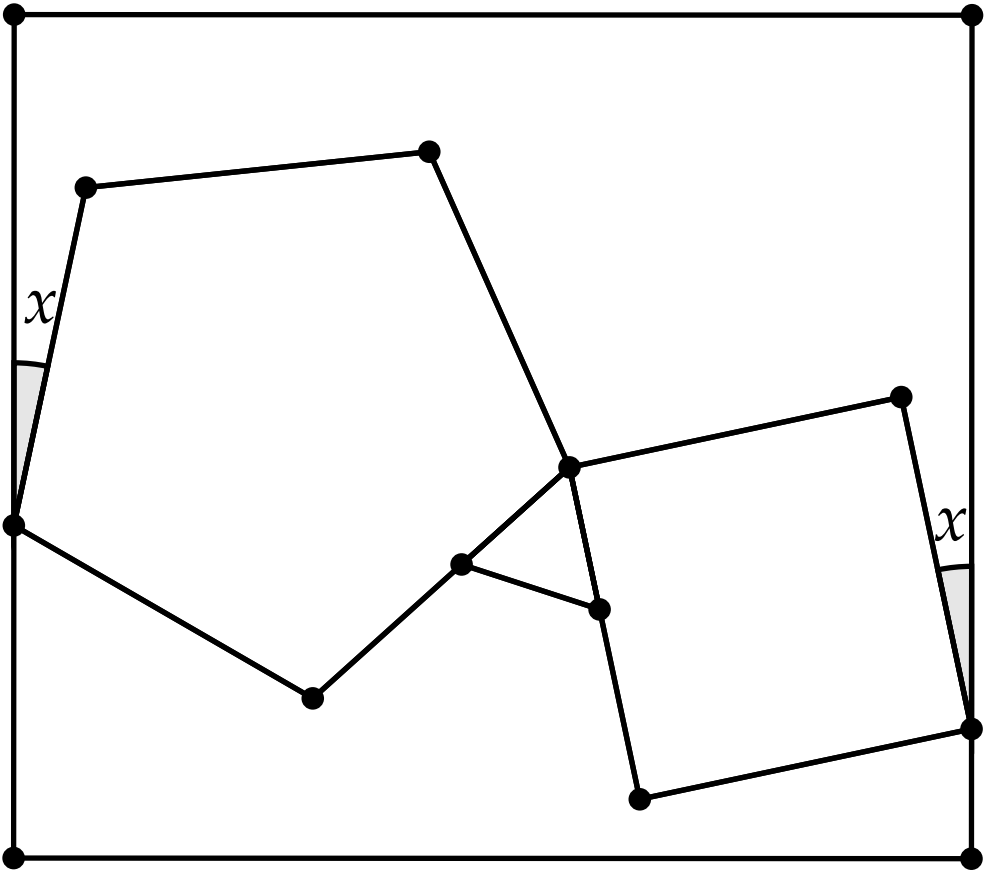
\includegraphics[width=0.4\textwidth]{second.png}
          \end{figure}

        \item Uma professora tem uma sala com menos de 100 alunos e possui 2024 balas para dar para eles. Ela gostaria
de distribuir uma quantidade igual de balas para cada aluno e observou que precisaria comprar no mínimo 41
balas para fazê-lo. Quantos alunos a sala possui?
        \item Em uma cidade com 2025 habitantes, cada pessoa sempre mente ou sempre fala a verdade. Um dia Ana,
          que é habitante desta cidade, faz o seguinte anúncio: “Nessa cidade há um número ímpar de mentirosos!”

          Considere as seguintes afirmações:
          \begin{enumerate}[label={\roman*.}]
            \item Ana sempre fala a verdade.
            \item Existe pelo menos um mentiroso na cidade.
            \item Existe pelo menos uma pessoa que diz a verdade na cidade.
            \item Existe pelo menos uma pessoa diferente de Ana que sempre diz a verdade na cidade.
          \end{enumerate}
          Quantas afirmações são necessariamente verdadeiras?
        \item O retângulo $ABCD$ possui lados com medidas $AB = 8$ e $BC = 4$. Os pontos $E$ e $F$ são pontos médios dos
lados $CD$ e $AB$, respectivamente. A reta $AE$ encontra a reta $BC$ em $G$ e a reta $GF$ encontra a reta $AD$ em $H$. Qual
é a área do triângulo $AGH$?
          \begin{figure}[h]
            \centering
            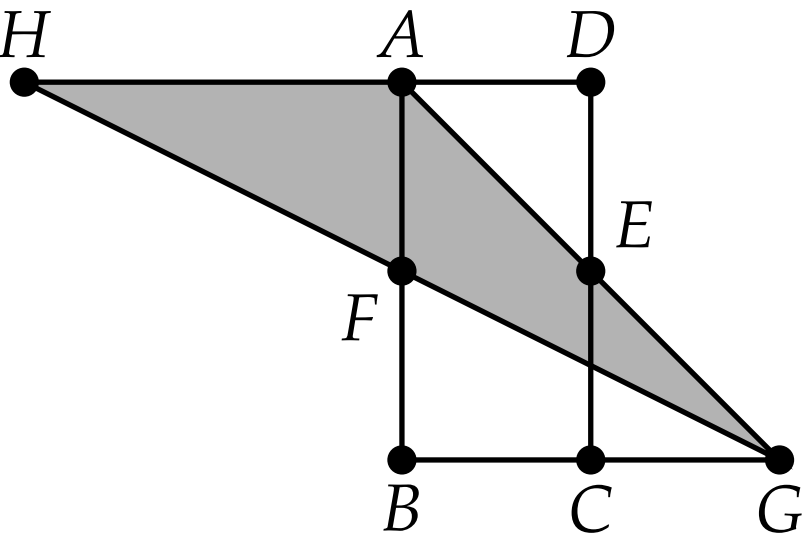
\includegraphics[width=0.3\textwidth]{third.png}
          \end{figure}
        \item No planeta Xorpzorp, as semanas têm $11$ dias (chamados de $1^a$ feira, \dots, $11^a$ feira); os meses alternam entre
$50$ e $51$ dias, e os anos têm exatamente $5$ meses, ou seja, alternam entre $252$ ou $253$ dias. Em Xorpzorp, um dia
tem a mesma duração de um dia terrestre.

Hoje, nesse planeta, é $4^a$ feira, dia $51$ do mês $4$ de $2024$. Daqui a $24$ anos terrestres, qual será o dia no calendário
Xorpzorp?
\item O triângulo $ABC$ é isósceles de base $BC$. Os pontos $E$ no segmento $AB$ e $F$, $G$ no segmento $AC$ satisfazem:
\begin{enumerate}[label={\roman*.}]
  \item $A$, $F$, $G$ e $C$ estão dispostos nessa ordem;
  \item $AF = EF$;
  \item $EF$ é bissetriz de $\angle AEG$;
  \item $GB$ é bissetriz de $\angle EGC$;
  \item $BC = BG$.
\end{enumerate}
Quanto vale o ângulo $\angle BAC$?
\item Maria escreveu no quadro branco os primeiros $1000$ múltiplos de $23$, começando com $23$ e em ordem
crescente. José, em seguida, apagou os dígitos a partir do quarto, em cada número (então $12345$ vira $345$).
Sobrou uma lista de $1000$ números de $3$ (ou menos) dígitos.

Entre as alternativas a seguir, qual delas aparece por último no quadro branco?
\item As circunferências $\omega_1$ de centro $A$ que passa por $B$ e $\omega_2$ de centro $B$ que passa por $A$ se encontram no ponto
$C$. A reta $BC$ corta $\omega_2$ novamente em $D$. A reta $DA$ corta $\omega_1$ em $E$ (o ponto $A$ está entre $D$ e $E$). Finalmente, a
reta $EB$ corta $\omega_2$ em $F$ (o ponto $B$ está entre $E$ e $F$). Determine a medida em graus do ângulo $\angle DEF$.
          \begin{figure}[h]
            \centering
            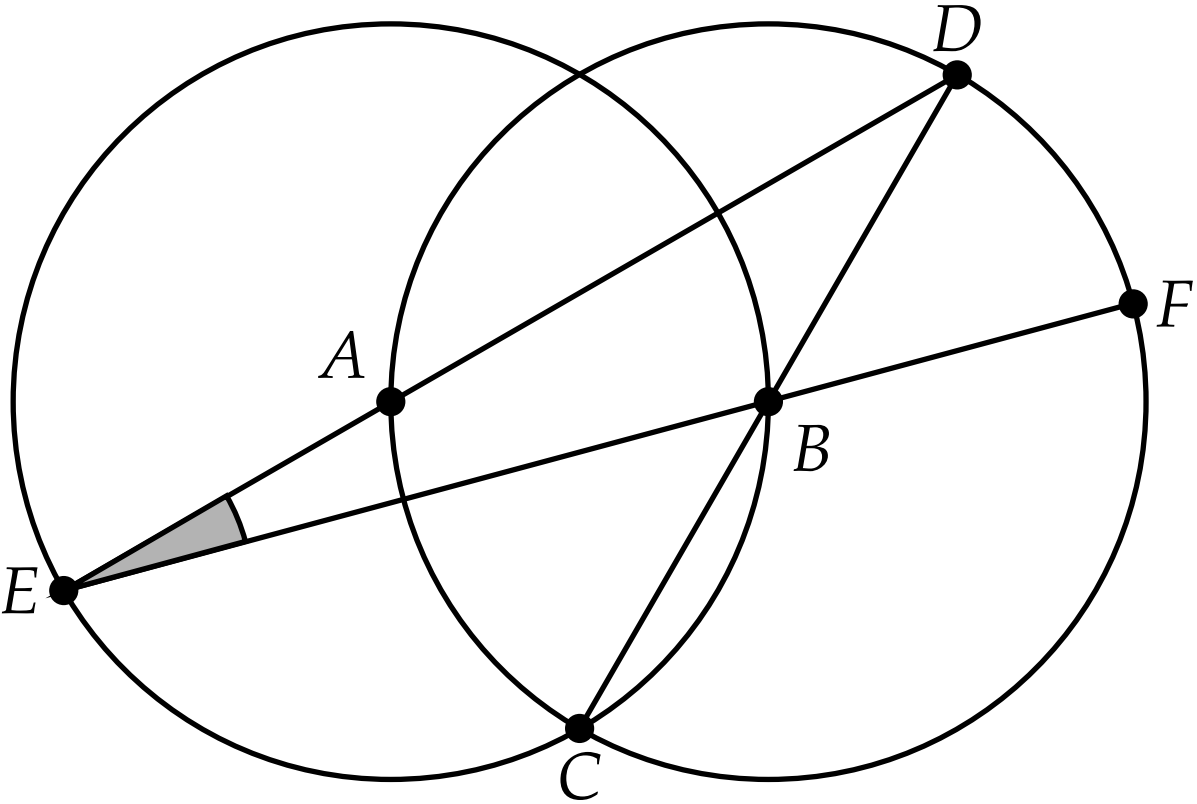
\includegraphics[width=0.5\textwidth]{fourth.png}
          \end{figure}
        \item De quantas maneiras podemos pintar os pontos $E$, $F$, $G$, $H$, $I$, $J$ da figura a seguir, cada um com exatamente
uma cor, se temos disponíveis as cores vermelho, verde e azul, e se não devemos permitir que três pontos
colineares recebam a mesma cor?

          \begin{figure}[h]
            \centering
            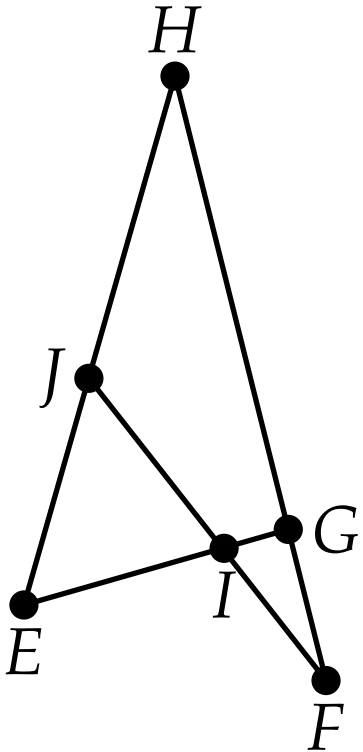
\includegraphics[width=0.15\textwidth]{fifth.png}
          \end{figure}
        \item O sistema
          \[
            \begin{cases}
              a^3 + b = 4c,\\
              a + b^3 = c,\\
              ab = -1
            \end{cases}
          \]
          tem solução real. Quantos valores de \(a\) satisfazem o sistema?
        \item Um tabuleiro \(15 \times 36\) será coberto, sem sobreposição, por peças quadradas de lado \(5 \times 5\) e \(7 \times 7\).
          Se nenhuma parte dessas peças pode ficar fora do tabuleiro, qual o número mínimo de quadradinhos que não serão cobertos?    
      \end{enumerate}
    \subsection{Respostas Numéricas}
      \begin{enumerate}[label=\textbf{\arabic*.}, start=16]
        \item Seja \(N\) um inteiro positivo de quatro algarismos cujo algarismo das unidades é igual a 3 e seja \(M\) o número obtido de
          \(N\) apagando esse algarismo 3 e escrevendo-o no começo de \(N\). Sabe-se que \(M\) é 2025 unidades menor que \(N\).Qual é o valor
          de \(N\)?
        \item Um número $a$ \textit{ganha} de outro $b$ se $a > b$ e o número obtido invertendo os dígitos de a na base decimal é
maior do que o número obtido invertendo os dígitos de $b$ na base decimal. Por exemplo, $314$ ganha de $291$,
pois $314 > 291$ e $413 > 192$. Por outro lado, $314$ não ganha de $309$, pois $413 < 903$.
Quantos números de quatro algarismos ganham de $2024$?
        \item Considere a expressão

          \begin{figure}[h]
            \centering
            
\includegraphics[width=0.25\textwidth]{seventh.png}
          \end{figure}
          Em cada espaço vazio, coloque um \(+\) ou um \(-\) e calcule o resultado. Quantos são os possíveis restos desse resultado na
          divisão por 2024?
        \item Sejam \(a,b,c\) tais que
          \[
            \begin{cases}
              a+b+c=10,\\
              a^2+b^2+c^2=20,\\
              a^3+b^3+c^3=30.
            \end{cases}
          \]
          Calcule o valor de \(a^5+b^5+c^5\).
        \item Na figura a seguir temos um paralelogramo em que cada lado foi dividido em três partes iguais. Os pontos sobre os lados foram
          ligados alternadamente para formar dois quadriláteros. A figura sombreada é formada pela união das regiões desses dois quadriláteros.
          A razão entre a área sombreada e a área do paralelogramo pode ser escrita como fração irredutível \(\tfrac{p}{q}\), com \(p,q\)
          inteiros positivos. Quanto vale \(p+q\)?
          \begin{figure}[h]
            \centering
            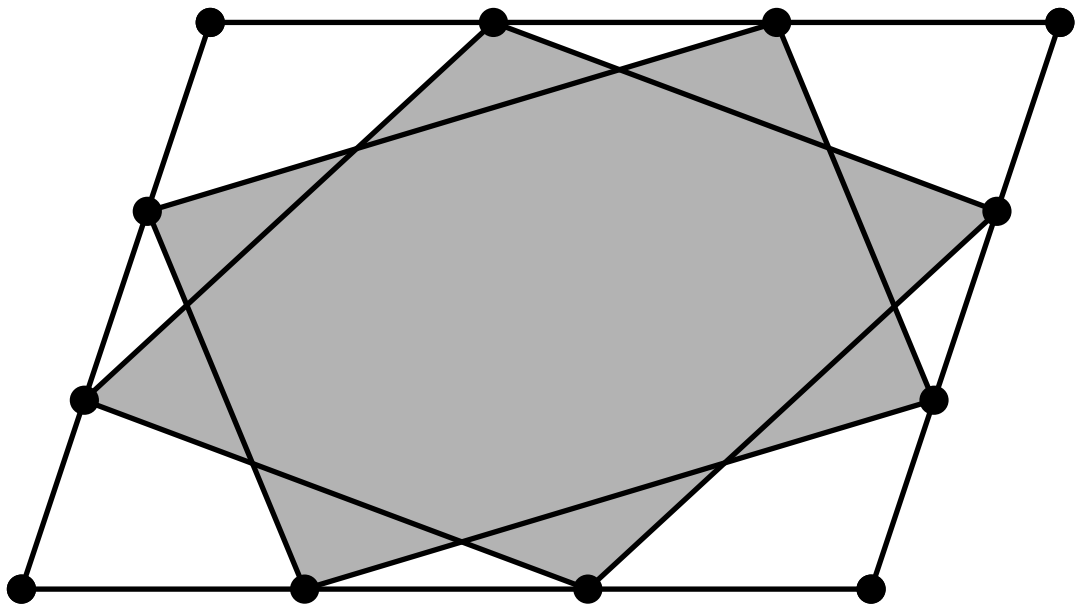
\includegraphics[width=0.4\textwidth]{sixth.png}
          \end{figure}
      \end{enumerate}
  \clearpage

  \section{\textsf{Soluções}}
  \subsection{Problema 1}
\begin{tcolorbox}[statementbox]
  Sejam \(x, y, z, w\) inteiros positivos tais que \(20^{24} = 2^x \cdot 5^y = 8^z \cdot 25^w\). Qual é o valor de \(x + y + z + w\)?
\end{tcolorbox}

\clearpage

\subsection{Problema 2}
\begin{tcolorbox}[statementbox]
Lucas estava participando de uma corrida de rua de 21 quilômetros e olhando sempre o tempo médio por quilômetro. Ao final do
quilômetro 14 o seu tempo médio era de 6 minutos e 42 segundos por quilômetro. Nos últimos 7 quilômetros o ritmo dele baixou e ele
concluiu o quilômetro 21 com tempo médio de 6 minutos e 50 segundos por quilômetro no percurso completo. Qual foi o tempo médio de
Lucas nos últimos 7 quilômetros?
\end{tcolorbox}

\clearpage

\subsection{Problema 3}
\begin{tcolorbox}[statementbox]
Qual o número máximo de meses com 5 quintas-feiras que um ano pode ter?
\end{tcolorbox}

\clearpage

\subsection{Problema 4}
\begin{tcolorbox}[statementbox]
Quantos triângulos na figura abaixo têm soma de seus números par?
\begin{center}
  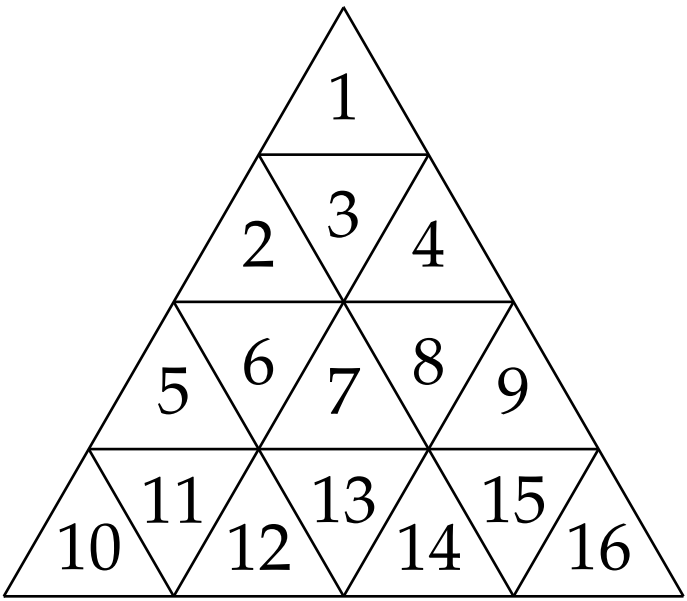
\includegraphics[width=0.25\textwidth]{first.png}
\end{center}
\end{tcolorbox}

\clearpage

\subsection{Problema 5}
\begin{tcolorbox}[statementbox]
Na figura a seguir no interior de um retângulo há um pentágono regular, um triângulo equilátero e um
quadrado. Os três polígonos regulares possuem um vértice em comum, os outros dois vértices do triângulo
equilátero estão sobre os lados do pentágono e do quadrado e o pentágono e o quadrado possuem um vértice
sobre os lados do retângulo. Sabe-se que lados do pentágono e do quadrado formam ângulos com medida x
com lados opostos do retângulo (como na figura). Quanto vale x em graus?
\begin{center}
  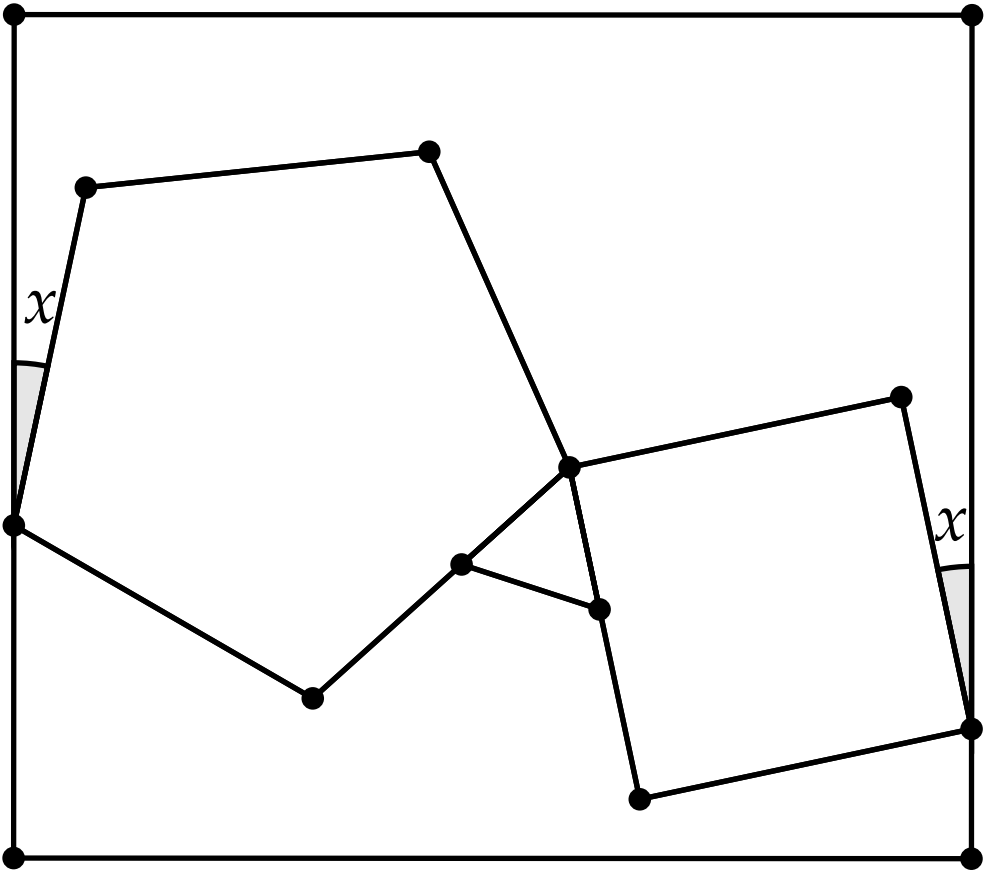
\includegraphics[width=0.4\textwidth]{second.png}
\end{center}
\end{tcolorbox}

\clearpage

\subsection{Problema 6}
\begin{tcolorbox}[statementbox]
Uma professora tem uma sala com menos de 100 alunos e possui 2024 balas para dar para eles. Ela gostaria
de distribuir uma quantidade igual de balas para cada aluno e observou que precisaria comprar no mínimo 41
balas para fazê-lo. Quantos alunos a sala possui?
\end{tcolorbox}

\clearpage

\subsection{Problema 7}
\begin{tcolorbox}[statementbox]
Em uma cidade com 2025 habitantes, cada pessoa sempre mente ou sempre fala a verdade. Um dia Ana,
          que é habitante desta cidade, faz o seguinte anúncio: “Nessa cidade há um número ímpar de mentirosos!”

          Considere as seguintes afirmações:
          \begin{enumerate}[label={\roman*.}]
            \item Ana sempre fala a verdade.
            \item Existe pelo menos um mentiroso na cidade.
            \item Existe pelo menos uma pessoa que diz a verdade na cidade.
            \item Existe pelo menos uma pessoa diferente de Ana que sempre diz a verdade na cidade.
          \end{enumerate}
          Quantas afirmações são necessariamente verdadeiras?
\end{tcolorbox}

\clearpage

\subsection{Problema 8}
\begin{tcolorbox}[statementbox]
O retângulo $ABCD$ possui lados com medidas $AB = 8$ e $BC = 4$. Os pontos $E$ e $F$ são pontos médios dos
lados $CD$ e $AB$, respectivamente. A reta $AE$ encontra a reta $BC$ em $G$ e a reta $GF$ encontra a reta $AD$ em $H$. Qual
é a área do triângulo $AGH$?
\begin{center}
  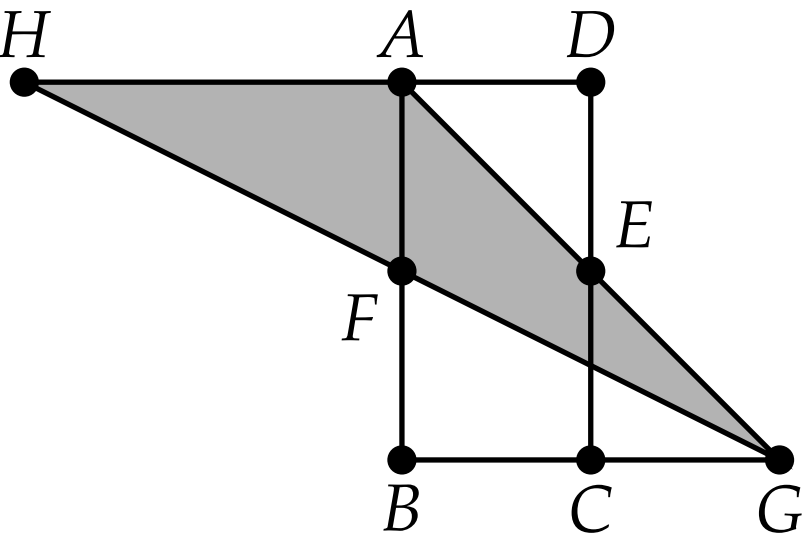
\includegraphics[width=0.4\textwidth]{third.png}
\end{center}
\end{tcolorbox}

\clearpage

\subsection{Problema 9}
\begin{tcolorbox}[statementbox]
No planeta Xorpzorp, as semanas têm $11$ dias (chamados de $1^a$ feira, \dots, $11^a$ feira); os meses alternam entre
$50$ e $51$ dias, e os anos têm exatamente $5$ meses, ou seja, alternam entre $252$ ou $253$ dias. Em Xorpzorp, um dia
tem a mesma duração de um dia terrestre.

Hoje, nesse planeta, é $4^a$ feira, dia $51$ do mês $4$ de $2024$. Daqui a $24$ anos terrestres, qual será o dia no calendário
Xorpzorp?
\end{tcolorbox}

\clearpage

\subsection{Problema 10}
\begin{tcolorbox}[statementbox]
O triângulo $ABC$ é isósceles de base $BC$. Os pontos $E$ no segmento $AB$ e $F$, $G$ no segmento $AC$ satisfazem:
\begin{enumerate}[label={\roman*.}]
  \item $A$, $F$, $G$ e $C$ estão dispostos nessa ordem;
  \item $AF = EF$;
  \item $EF$ é bissetriz de $\angle AEG$;
  \item $GB$ é bissetriz de $\angle EGC$;
  \item $BC = BG$.
\end{enumerate}
Quanto vale o ângulo $\angle BAC$?
\end{tcolorbox}

\clearpage

\subsection{Problema 11}
\begin{tcolorbox}[statementbox]
Maria escreveu no quadro branco os primeiros $1000$ múltiplos de $23$, começando com $23$ e em ordem
crescente. José, em seguida, apagou os dígitos a partir do quarto, em cada número (então $12345$ vira $345$).
Sobrou uma lista de $1000$ números de $3$ (ou menos) dígitos.
Entre as alternativas a seguir, qual delas aparece por último no quadro branco?

\end{tcolorbox}

\clearpage

\subsection{Problema 12}
\begin{tcolorbox}[statementbox]
As circunferências $\omega_1$ de centro $A$ que passa por $B$ e $\omega_2$ de centro $B$ que passa por $A$ se encontram no ponto
$C$. A reta $BC$ corta $\omega_2$ novamente em $D$. A reta $DA$ corta $\omega_1$ em $E$ (o ponto $A$ está entre $D$ e $E$). Finalmente, a
reta $EB$ corta $\omega_2$ em $F$ (o ponto $B$ está entre $E$ e $F$). Determine a medida em graus do ângulo $\angle DEF$.
          \begin{figure}[h]
            \centering
            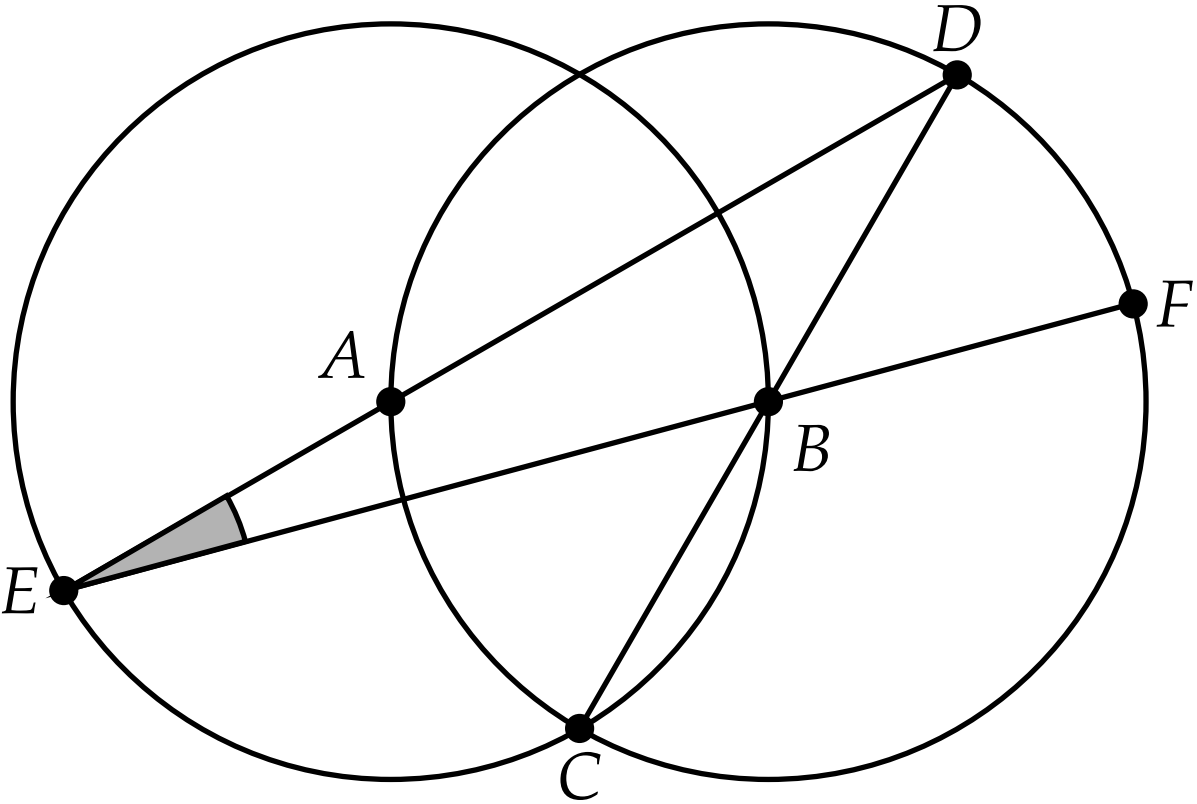
\includegraphics[width=0.5\textwidth]{fourth.png}
          \end{figure}
\end{tcolorbox}

\clearpage

\subsection{Problema 13}
\begin{tcolorbox}[statementbox]
  De quantas maneiras podemos pintar os pontos $E$, $F$, $G$, $H$, $I$, $J$ da figura a seguir, cada um com exatamente
uma cor, se temos disponíveis as cores vermelho, verde e azul, e se não devemos permitir que três pontos
colineares recebam a mesma cor?
\begin{center}
  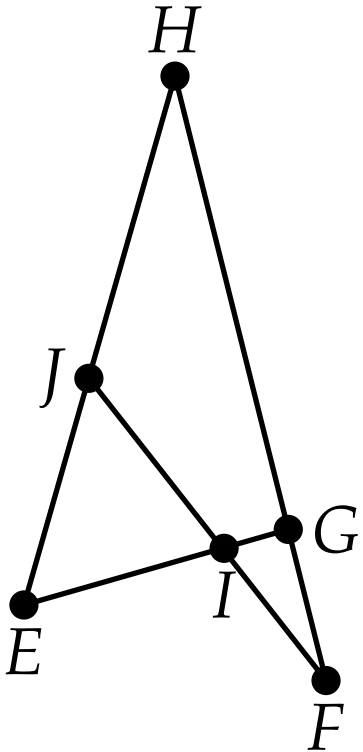
\includegraphics[width=0.15\textwidth]{fifth.png}
\end{center}
\end{tcolorbox}

\clearpage

\subsection{Problema 14}
\begin{tcolorbox}[statementbox]
O sistema
\[
  \begin{cases}
    a^3 + b = 4c,\\
    a + b^3 = c,\\
    ab = -1
  \end{cases}
\]
tem solução real. Quantos valores de \(a\) satisfazem o sistema?
\end{tcolorbox}

\clearpage

\subsection{Problema 15}
\begin{tcolorbox}[statementbox]
Um tabuleiro \(15 \times 36\) será coberto, sem sobreposição, por quadrados de lado \(5 \times 5\) e \(7 \times 7\). Nenhuma
parte das peças pode sair do tabuleiro. Qual é o número mínimo de quadradinhos que permanecerão descobertos?
\end{tcolorbox}

\clearpage

\subsection{Problema 16}
\begin{tcolorbox}[statementbox]
Seja \(N\) um inteiro positivo de quatro algarismos cujo algarismo das unidades é igual a 3 e seja \(M\) o número obtido de
\(N\) apagando esse algarismo 3 e escrevendo-o no começo de \(N\). Sabe-se que \(M\) é 2025 unidades menor que \(N\). Qual é o valor
de \(N\)?
\end{tcolorbox}

\clearpage

\subsection{Problema 17}
\begin{tcolorbox}[statementbox]
Um número $a$ \textit{ganha} de outro $b$ se $a > b$ e o número obtido invertendo os dígitos de a na base decimal é
maior do que o número obtido invertendo os dígitos de $b$ na base decimal. Por exemplo, $314$ ganha de $291$,
pois $314 > 291$ e $413 > 192$. Por outro lado, $314$ não ganha de $309$, pois $413 < 903$.
Quantos números de quatro algarismos ganham de $2024$?
\end{tcolorbox}

\clearpage

\subsection{Problema 18}
\begin{tcolorbox}[statementbox]
   Considere a expressão

          \begin{center}
            
\includegraphics[width=0.25\textwidth]{seventh.png}
          \end{center}
          Em cada espaço vazio, coloque um \(+\) ou um \(-\) e calcule o resultado. Quantos são os possíveis restos desse resultado na
          divisão por 2024?
\end{tcolorbox}

\clearpage

\subsection{Problema 19}
\begin{tcolorbox}[statementbox]
Sejam \(a,b,c\) tais que
\[
  \begin{cases}
    a+b+c=10,\\
    a^2+b^2+c^2=20,\\
    a^3+b^3+c^3=30.
  \end{cases}
\]
Calcule o valor de \(a^5+b^5+c^5\).
\end{tcolorbox}

\clearpage

\subsection{Problema 20}
\begin{tcolorbox}[statementbox]
Na figura a seguir temos um paralelogramo em que cada lado foi dividido em três partes iguais. Os pontos sobre os lados foram
ligados alternadamente para formar dois quadriláteros. A figura sombreada é formada pela união das regiões desses dois quadriláteros.
A razão entre a área sombreada e a área do paralelogramo pode ser escrita como fração irredutível \(\tfrac{p}{q}\), com \(p,q\)
inteiros positivos. Quanto vale \(p+q\)?
\begin{center}
  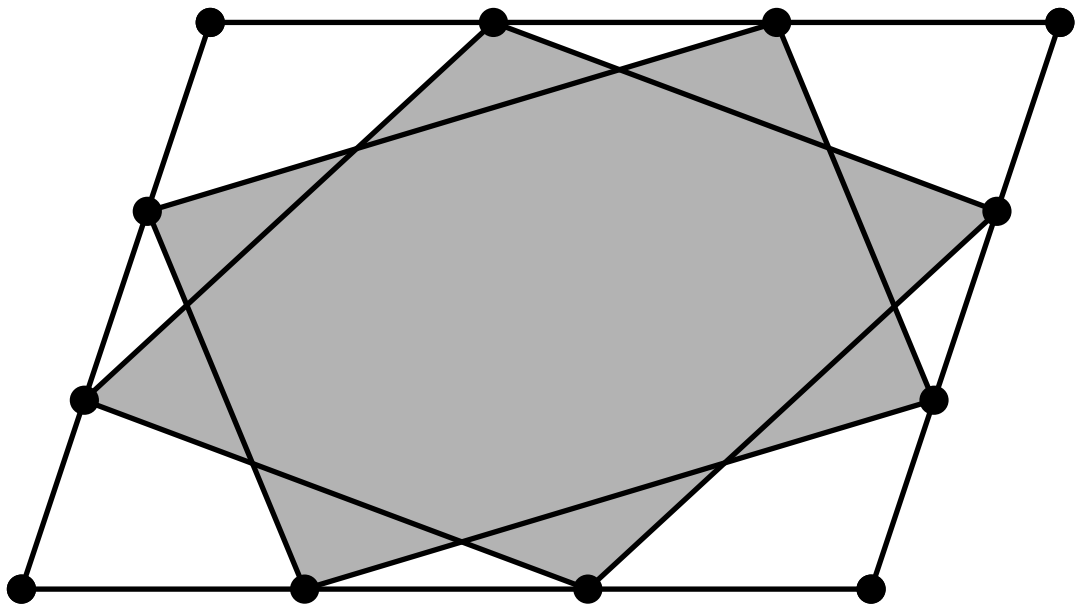
\includegraphics[width=0.4\textwidth]{sixth.png}
\end{center}
\end{tcolorbox}

  \clearpage

  \section{\textsf{Referências}}
\end{document}
